\subsection{Self-speed Estimator}
\label{sec:self-speed_estimator}
The vehicle's self-speed plays a crucial role in distinguishing between stationary and moving objects, as it enables the removal of dynamic points in later stages of the pipeline. 
It therefore needs to be determined in a reliable way.
Traditional approaches usually utilize external sensors such as wheel encoders, Global Positioning System (GPS), or Inertia Measurement Units (IMUs).
In this project, a technique was developed that determines the vehicle's self-speed only by processing the point cloud's data.
An angle $\phi_{p}$ was defined between each individual point of the point cloud and the radar sensor's centerline:
\par
\begin{figure}[!htbp]
    \centering
    %\resizebox{0.48\textwidth}{!}{
        \begin{tikzpicture}
            \gokart{0}{0}{0}

            \coordinate(O) at (0,0);
            \coordinate(P) at (0.75,1.5);
            \coordinate(A) at (0,1.5);

            \draw[dashed, thick, gray] ($(P)!1.2!(O)$) -- ($(O)!1.2!(P)$);
            \draw[dashed, thick] ($(A)!1.2!(O)$) -- ($(O)!1.24!(A)$);
            \draw pic["$\phi_{p}$", draw=black, angle radius=1.68cm, angle eccentricity=0.85] {angle=P--O--A};
            \draw[fill=red] (P) circle (0.07) node [right] {\small $p$};

            \draw[->, thick, red] (-0.2,0) -- (0.4,0) node[above] {\small $x$};
            \draw[->, thick, red] (0,-0.2) -- (0,0.4) node[left] {\small $y$};
            \fill[red] (0,0) circle (0.05);
        \end{tikzpicture}
    %}
    \caption{Definition of the angle $\phi_{p}$}
    \label{fig:def_angle_phi}
\end{figure}
\FloatBarrier\noindent

\subsubsection*{Scalar Ego-Speed Estimation}
The first stage estimates the forward speed of the vehicle under the assumption of motion along the $+y$ axis. 
For each radar detection, the angle $\phi_p$ relative to the sensor's forward axis is defined (see Figure~\ref{fig:def_angle_phi}):  

\[
\phi_{p} = \arctan\left(\frac{x_p}{y_p}\right).
\]

The observed radial velocity of a static point $p$ depends on the vehicle speed $v_0$ and follows a cosine law:  

\[
v_{r,p}(v_0,\phi_p) = -v_0 \cdot \cos(\phi_p).
\]

Since no point lies exactly on $\phi=0^\circ$ and noise is present, all available inlier points (after RANSAC filtering) are used to fit a regression curve $v(\phi)$ to the measured pairs $(\phi_p, v_{r,p})$. 
The fitted value at $\phi = 0^\circ$ provides the best estimate of the scalar vehicle speed. 
A least-squares polynomial regression of order 2 is sufficient, since $\cos(\phi)$ can be locally approximated in the domain $\phi_p \in \left[-\frac{\pi}{2}, \frac{\pi}{2}\right]$ by:  

\[
\cos(\phi_p) \approx a \phi_p^2 + b.
\]

\subsubsection*{Generalized 2D Ego-Velocity Estimation}
The scalar approach assumes purely forward motion. 
To extend the model, the Doppler equation for a static point observed at angle $\theta$ is introduced:  

\[
v_{r}(\theta) = v_x \cos(\theta) + v_y \sin(\theta),
\]

where $v_x$ and $v_y$ are the ego-velocity components along the $x$ and $y$ axes of the vehicle frame.  
This equation is linear in $v_x$ and $v_y$, which allows solving for both components simultaneously using a least-squares approach across multiple points:  

\[
\begin{bmatrix}
v_{r,1} \\
v_{r,2} \\
\vdots \\
v_{r,n}
\end{bmatrix}
=
\begin{bmatrix}
\cos(\theta_1) & \sin(\theta_1) \\
\cos(\theta_2) & \sin(\theta_2) \\
\vdots & \vdots \\
\cos(\theta_n) & \sin(\theta_n)
\end{bmatrix}
\begin{bmatrix}
v_x \\ v_y
\end{bmatrix}.
\]

This formulation naturally integrates into the existing pipeline: RANSAC provides inlier points representing static structures, and the least-squares solution yields robust estimates of both forward and lateral velocity components.  

\subsubsection*{Practical Considerations}
Test runs demonstrated that the radar-only ego-velocity estimate closely followed the reference vehicle speed with a small static offset. 
However, fluctuations occurred in cases with sparse point clouds. 
This effect was mitigated by tuning the frame aggregation window and applying a Kalman filter after the regression stage, providing a stable and continuous self-speed estimate for downstream filtering and odometry estimation.  

\begin{figure}[!htbp]
    \centering
    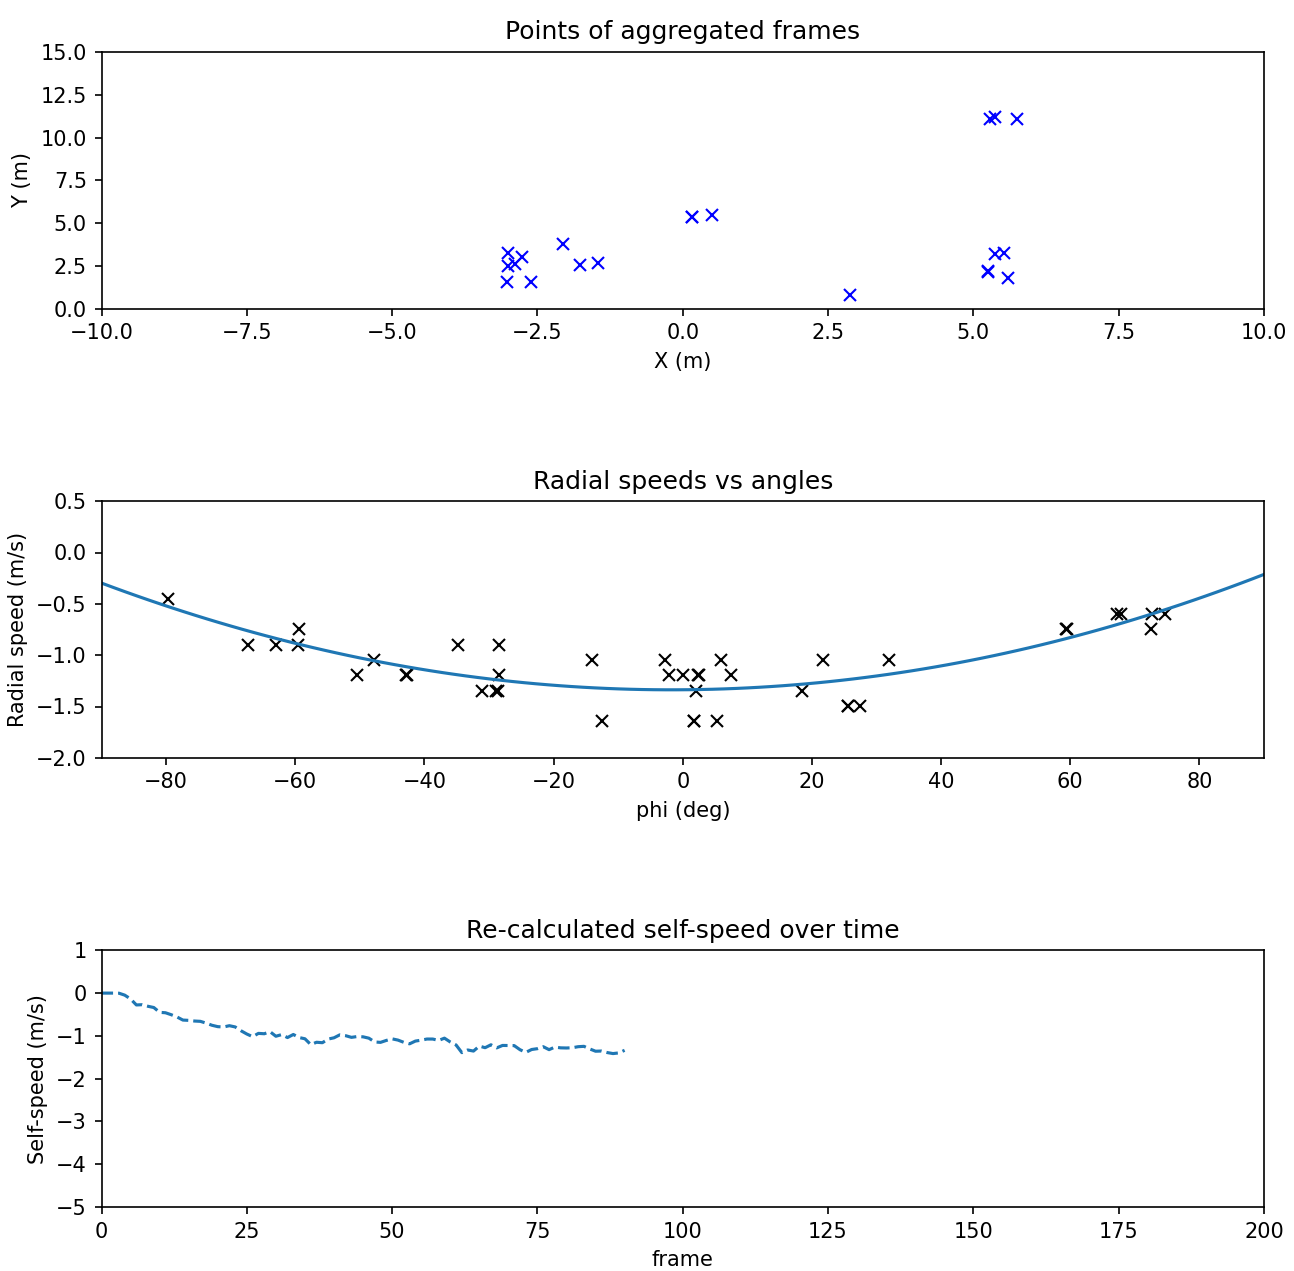
\includegraphics[width=1.0\linewidth]{images/self_speed_reality.png}
    \caption{Example of radar-based self-speed estimation compared against the ground truth indicator.}
    \label{fig:self_speed_test_data}
\end{figure}

\FloatBarrier\noindent
The full process of ego-velocity estimation is summarized in Figure~\ref{fig:self_speed_block}. 
The radar point cloud is first filtered using RANSAC to retain only inliers corresponding to static structures. 
From these points, both the azimuth angle and Doppler velocity are extracted. 
At this stage, the pipeline branches into two estimation strategies:  

\begin{itemize}
    \item \textbf{Scalar ego-speed estimation:} a polynomial regression approximates the cosine law of Doppler velocities, yielding the forward velocity component only.
    \item \textbf{2D ego-velocity estimation:} a linear least-squares solution of the Doppler equation
    \[
    v_{r}(\theta) = v_x \cos(\theta) + v_y \sin(\theta)
    \]
    provides both longitudinal ($v_y$) and lateral ($v_x$) velocity components simultaneously.
\end{itemize}

Both outputs are subsequently passed through a Kalman filter for temporal smoothing before being used in the downstream pipeline.

\begin{figure}[!htbp]
    \centering
    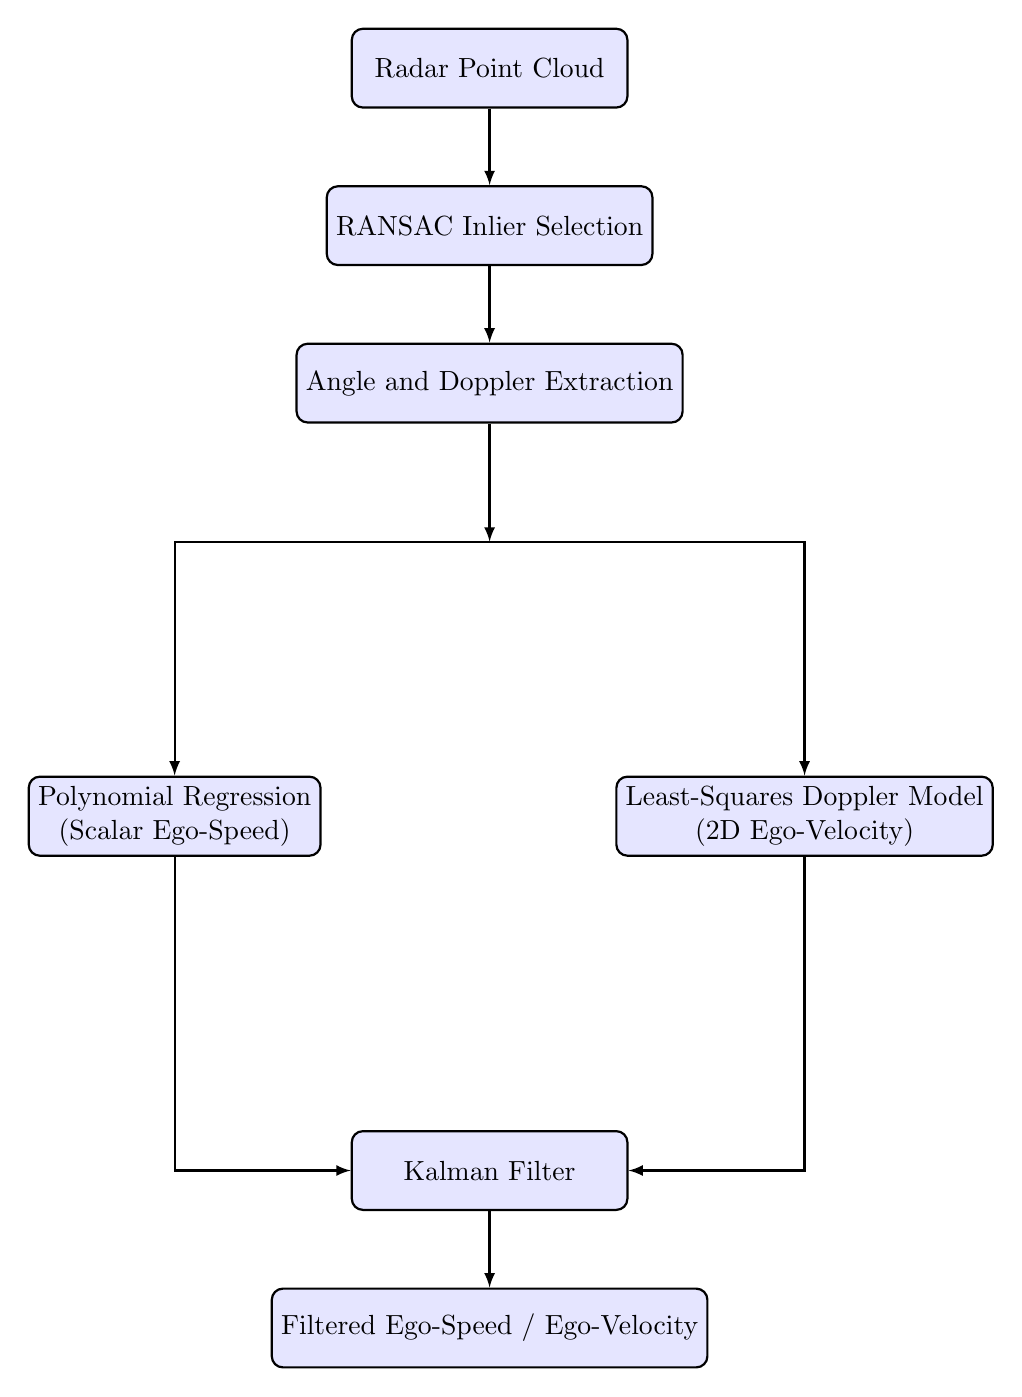
\begin{tikzpicture}[node distance=2cm,>=latex,thick]
        \tikzstyle{block} = [rectangle, draw, fill=blue!10, text centered, rounded corners, minimum height=1cm, minimum width=3.5cm, align=center]
        \tikzstyle{arrow} = [->, thick]

        % Nodes
        \node[block] (input) {Radar Point Cloud};
        \node[block, below of=input] (ransac) {RANSAC Inlier Selection};
        \node[block, below of=ransac] (angles) {Angle and Doppler Extraction};

        % Branch nodes
        \node[block, below of=angles, xshift=-4cm, yshift=-3.5cm] (scalar) {\shortstack{Polynomial Regression \\ (Scalar Ego-Speed)}};
        \node[block, below of=angles, xshift=4cm, yshift=-3.5cm] (vector) {\shortstack{Least-Squares Doppler Model \\ (2D Ego-Velocity)}};

        % Output and filter
        \node[block, below of=angles, yshift=-8cm] (kalman) {Kalman Filter};
        \node[block, below of=kalman] (output) {Filtered Ego-Speed / Ego-Velocity};

        % Straight arrows
        \draw[arrow] (input) -- (ransac);
        \draw[arrow] (ransac) -- (angles);

        % Branching arrows (down, then sideways)
        \draw[arrow] (angles.south) -- ++(0,-1.5) coordinate(branch);
        \draw[arrow] (branch) -| (scalar.north);
        \draw[arrow] (branch) -| (vector.north);

        % Merge arrows (sideways, then down)
        \draw[arrow] (scalar.south) |- (kalman.west);
        \draw[arrow] (vector.south) |- (kalman.east);

        % Final output
        \draw[arrow] (kalman) -- (output);
    \end{tikzpicture}
    \caption{Block diagram of the self-speed estimation process, showing the two complementary approaches: scalar polynomial fitting and 2D Doppler-based least-squares estimation.}
    \label{fig:self_speed_block}
\end{figure}

